% Options for packages loaded elsewhere
\PassOptionsToPackage{unicode}{hyperref}
\PassOptionsToPackage{hyphens}{url}
\PassOptionsToPackage{dvipsnames,svgnames,x11names}{xcolor}
%
\documentclass[
  11pt,
]{krantz}
\usepackage{amsmath,amssymb}
\usepackage{lmodern}
\usepackage{iftex}
\ifPDFTeX
  \usepackage[T1]{fontenc}
  \usepackage[utf8]{inputenc}
  \usepackage{textcomp} % provide euro and other symbols
\else % if luatex or xetex
  \usepackage{unicode-math}
  \defaultfontfeatures{Scale=MatchLowercase}
  \defaultfontfeatures[\rmfamily]{Ligatures=TeX,Scale=1}
  \setmonofont[Scale=0.775]{MesloLGS NF}
\fi
% Use upquote if available, for straight quotes in verbatim environments
\IfFileExists{upquote.sty}{\usepackage{upquote}}{}
\IfFileExists{microtype.sty}{% use microtype if available
  \usepackage[]{microtype}
  \UseMicrotypeSet[protrusion]{basicmath} % disable protrusion for tt fonts
}{}
\makeatletter
\@ifundefined{KOMAClassName}{% if non-KOMA class
  \IfFileExists{parskip.sty}{%
    \usepackage{parskip}
  }{% else
    \setlength{\parindent}{0pt}
    \setlength{\parskip}{6pt plus 2pt minus 1pt}}
}{% if KOMA class
  \KOMAoptions{parskip=half}}
\makeatother
\usepackage{xcolor}
\IfFileExists{xurl.sty}{\usepackage{xurl}}{} % add URL line breaks if available
\IfFileExists{bookmark.sty}{\usepackage{bookmark}}{\usepackage{hyperref}}
\hypersetup{
  pdftitle={Data Science per psicologi},
  pdfauthor={Corrado Caudek},
  colorlinks=true,
  linkcolor={Maroon},
  filecolor={Maroon},
  citecolor={Blue},
  urlcolor={Blue},
  pdfcreator={LaTeX via pandoc}}
\urlstyle{same} % disable monospaced font for URLs
\usepackage{color}
\usepackage{fancyvrb}
\newcommand{\VerbBar}{|}
\newcommand{\VERB}{\Verb[commandchars=\\\{\}]}
\DefineVerbatimEnvironment{Highlighting}{Verbatim}{commandchars=\\\{\}}
% Add ',fontsize=\small' for more characters per line
\usepackage{framed}
\definecolor{shadecolor}{RGB}{248,248,248}
\newenvironment{Shaded}{\begin{snugshade}}{\end{snugshade}}
\newcommand{\AlertTok}[1]{\textcolor[rgb]{0.33,0.33,0.33}{#1}}
\newcommand{\AnnotationTok}[1]{\textcolor[rgb]{0.37,0.37,0.37}{\textbf{\textit{#1}}}}
\newcommand{\AttributeTok}[1]{\textcolor[rgb]{0.61,0.61,0.61}{#1}}
\newcommand{\BaseNTok}[1]{\textcolor[rgb]{0.06,0.06,0.06}{#1}}
\newcommand{\BuiltInTok}[1]{#1}
\newcommand{\CharTok}[1]{\textcolor[rgb]{0.5,0.5,0.5}{#1}}
\newcommand{\CommentTok}[1]{\textcolor[rgb]{0.37,0.37,0.37}{\textit{#1}}}
\newcommand{\CommentVarTok}[1]{\textcolor[rgb]{0.37,0.37,0.37}{\textbf{\textit{#1}}}}
\newcommand{\ConstantTok}[1]{\textcolor[rgb]{0,0,0}{#1}}
\newcommand{\ControlFlowTok}[1]{\textcolor[rgb]{0.27,0.27,0.27}{\textbf{#1}}}
\newcommand{\DataTypeTok}[1]{\textcolor[rgb]{0.27,0.27,0.27}{#1}}
\newcommand{\DecValTok}[1]{\textcolor[rgb]{0.06,0.06,0.06}{#1}}
\newcommand{\DocumentationTok}[1]{\textcolor[rgb]{0.37,0.37,0.37}{\textbf{\textit{#1}}}}
\newcommand{\ErrorTok}[1]{\textcolor[rgb]{0.14,0.14,0.14}{\textbf{#1}}}
\newcommand{\ExtensionTok}[1]{#1}
\newcommand{\FloatTok}[1]{\textcolor[rgb]{0.06,0.06,0.06}{#1}}
\newcommand{\FunctionTok}[1]{\textcolor[rgb]{0,0,0}{#1}}
\newcommand{\ImportTok}[1]{#1}
\newcommand{\InformationTok}[1]{\textcolor[rgb]{0.37,0.37,0.37}{\textbf{\textit{#1}}}}
\newcommand{\KeywordTok}[1]{\textcolor[rgb]{0.27,0.27,0.27}{\textbf{#1}}}
\newcommand{\NormalTok}[1]{#1}
\newcommand{\OperatorTok}[1]{\textcolor[rgb]{0.43,0.43,0.43}{\textbf{#1}}}
\newcommand{\OtherTok}[1]{\textcolor[rgb]{0.37,0.37,0.37}{#1}}
\newcommand{\PreprocessorTok}[1]{\textcolor[rgb]{0.37,0.37,0.37}{\textit{#1}}}
\newcommand{\RegionMarkerTok}[1]{#1}
\newcommand{\SpecialCharTok}[1]{\textcolor[rgb]{0,0,0}{#1}}
\newcommand{\SpecialStringTok}[1]{\textcolor[rgb]{0.5,0.5,0.5}{#1}}
\newcommand{\StringTok}[1]{\textcolor[rgb]{0.5,0.5,0.5}{#1}}
\newcommand{\VariableTok}[1]{\textcolor[rgb]{0,0,0}{#1}}
\newcommand{\VerbatimStringTok}[1]{\textcolor[rgb]{0.5,0.5,0.5}{#1}}
\newcommand{\WarningTok}[1]{\textcolor[rgb]{0.37,0.37,0.37}{\textbf{\textit{#1}}}}
\usepackage{longtable,booktabs,array}
\usepackage{calc} % for calculating minipage widths
% Correct order of tables after \paragraph or \subparagraph
\usepackage{etoolbox}
\makeatletter
\patchcmd\longtable{\par}{\if@noskipsec\mbox{}\fi\par}{}{}
\makeatother
% Allow footnotes in longtable head/foot
\IfFileExists{footnotehyper.sty}{\usepackage{footnotehyper}}{\usepackage{footnote}}
\makesavenoteenv{longtable}
\usepackage{graphicx}
\makeatletter
\def\maxwidth{\ifdim\Gin@nat@width>\linewidth\linewidth\else\Gin@nat@width\fi}
\def\maxheight{\ifdim\Gin@nat@height>\textheight\textheight\else\Gin@nat@height\fi}
\makeatother
% Scale images if necessary, so that they will not overflow the page
% margins by default, and it is still possible to overwrite the defaults
% using explicit options in \includegraphics[width, height, ...]{}
\setkeys{Gin}{width=\maxwidth,height=\maxheight,keepaspectratio}
% Set default figure placement to htbp
\makeatletter
\def\fps@figure{htbp}
\makeatother
\setlength{\emergencystretch}{3em} % prevent overfull lines
\providecommand{\tightlist}{%
  \setlength{\itemsep}{0pt}\setlength{\parskip}{0pt}}
\setcounter{secnumdepth}{5}
\usepackage{amsmath}
\usepackage{amssymb}
\usepackage{amsfonts}

\defaultfontfeatures{Scale=MatchLowercase}

\usepackage{booktabs}
\usepackage{longtable}
\usepackage[bf,singlelinecheck=off]{caption}

\usepackage{framed,color}
\definecolor{shadecolor}{RGB}{248,248,248}

\renewcommand{\textfraction}{0.05}
\renewcommand{\topfraction}{0.8}
\renewcommand{\bottomfraction}{0.8}
\renewcommand{\floatpagefraction}{0.75}

\renewenvironment{quote}{\begin{VF}}{\end{VF}}
\let\oldhref\href
\renewcommand{\href}[2]{#2\footnote{\url{#1}}}

\ifxetex
  \usepackage{letltxmacro}
  \setlength{\XeTeXLinkMargin}{1pt}
  \LetLtxMacro\SavedIncludeGraphics\includegraphics
  \def\includegraphics#1#{% #1 catches optional stuff (star/opt. arg.)
    \IncludeGraphicsAux{#1}%
  }%
  \newcommand*{\IncludeGraphicsAux}[2]{%
    \XeTeXLinkBox{%
      \SavedIncludeGraphics#1{#2}%
    }%
  }%
\fi

\makeatletter
\newenvironment{kframe}{%
\medskip{}
\setlength{\fboxsep}{.8em}
 \def\at@end@of@kframe{}%
 \ifinner\ifhmode%
  \def\at@end@of@kframe{\end{minipage}}%
  \begin{minipage}{\columnwidth}%
 \fi\fi%
 \def\FrameCommand##1{\hskip\@totalleftmargin \hskip-\fboxsep
 \colorbox{shadecolor}{##1}\hskip-\fboxsep
     % There is no \\@totalrightmargin, so:
     \hskip-\linewidth \hskip-\@totalleftmargin \hskip\columnwidth}%
 \MakeFramed {\advance\hsize-\width
   \@totalleftmargin\z@ \linewidth\hsize
   \@setminipage}}%
 {\par\unskip\endMakeFramed%
 \at@end@of@kframe}
\makeatother

\renewenvironment{Shaded}{\begin{kframe}}{\end{kframe}}

\usepackage{makeidx}
\makeindex

\urlstyle{tt}

\usepackage{amsthm}
\makeatletter
\def\thm@space@setup{%
  \thm@preskip=8pt plus 2pt minus 4pt
  \thm@postskip=\thm@preskip
}
\makeatother

\DeclareMathOperator{\V}{\mathbb{V}} % Define variance operator
\DeclareMathOperator{\Var}{\mathbb{V}} % Define variance operator
\DeclareMathOperator{\SD}{SD} % Define sd operator
\DeclareMathOperator{\Cov}{Cov} % Define covariance operator
\DeclareMathOperator{\Corr}{Corr} % Define correlation operator
\DeclareMathOperator{\Me}{Me} % Define mediane operator
\DeclareMathOperator{\Mo}{Mo} % Define mode operator

\DeclareMathOperator{\Bin}{Binomial} % Define binomial operator
\DeclareMathOperator{\Bernoulli}{Bernoulli} % Define Bernoulli operator
\DeclareMathOperator{\Ber}{\mathscr{B}} % Define Bernoulli operator
\DeclareMathOperator{\Poi}{Poisson} % Define Poisson operator
\DeclareMathOperator{\Uniform}{Uniform} % Define Uniform operator
\DeclareMathOperator{\Cauchy}{Cauchy} % Define Cauchy operator
\DeclareMathOperator{\B}{B} % beta function
% \mbox{B}(a, b) % beta function
% \mbox{Beta}(a, b) % beta distribution

\DeclareMathOperator{\elpd}{elpd} % Define elpd operator
\DeclareMathOperator{\lppd}{lppd} % Define lppd operator
\DeclareMathOperator{\LOO}{LOO} % Define LOO operator
\DeclareMathOperator{\argmin}{arg\,min} 
\DeclareMathOperator{\argmax}{arg\,max} 

\newcommand{\E}{\mathbb{E}} % Define expected value operator
\newcommand{\R}{\textsf{R}} % Define R programming language symbol
\newcommand{\Real}{\mathbb{R}} % Define real number operator
\newcommand{\Prob}{\mathscr{P}}
\newcommand{\indep}{\perp \!\!\! \perp}

\usepackage[
 labelfont=bf,
 font={small, it}
]{caption}
\usepackage{upquote} % print correct quotes in verbatim-environments
\usepackage{empheq}
\usepackage{xfrac}

\usepackage{polyglossia}
\setmainlanguage{italian}

\frontmatter
\ifLuaTeX
  \usepackage{selnolig}  % disable illegal ligatures
\fi
\usepackage[]{natbib}
\bibliographystyle{apalike}

\title{Data Science per psicologi}
\author{Corrado Caudek}
\date{2022-02-10}

\usepackage{amsthm}
\newtheorem{theorem}{Teorema}[chapter]
\newtheorem{lemma}{Lemma}[chapter]
\newtheorem{corollary}{Corollario}[chapter]
\newtheorem{proposition}{Proposizione}[chapter]
\newtheorem{conjecture}{Congettura}[chapter]
\theoremstyle{definition}
\newtheorem{definition}{Definizione}[chapter]
\theoremstyle{definition}
\newtheorem{example}{Esempio}[chapter]
\theoremstyle{definition}
\newtheorem{exercise}{Esercizio}[chapter]
\theoremstyle{definition}
\newtheorem{hypothesis}{Hypothesis}[chapter]
\theoremstyle{remark}
\newtheorem*{remark}{Osservazione}
\newtheorem*{solution}{Soluzione}
\begin{document}
\maketitle

\cleardoublepage\newpage\thispagestyle{empty}\null
% \cleardoublepage\newpage\thispagestyle{empty}\null
%\cleardoublepage\newpage
\thispagestyle{empty}
\begin{center}
\Large{Psicometria -- AA 2021/2022}

\vskip20pt

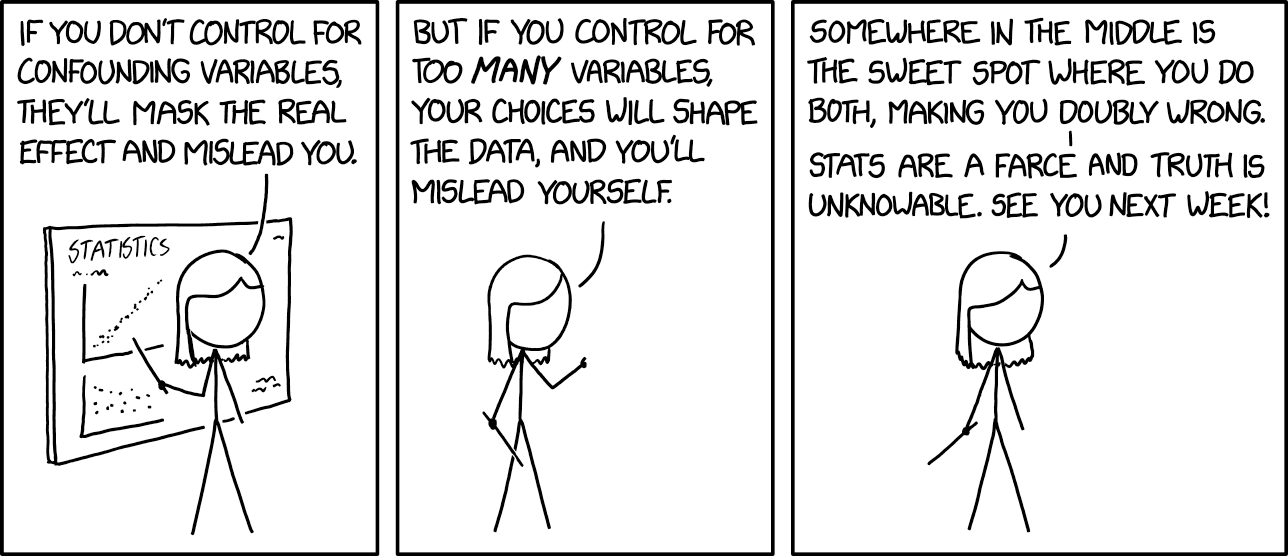
\includegraphics{images/confounding_variables.png}
\end{center}

\setlength{\abovedisplayskip}{-5pt}
\setlength{\abovedisplayshortskip}{-5pt}

{
\hypersetup{linkcolor=}
\setcounter{tocdepth}{2}
\tableofcontents
}
\listoffigures
\listoftables
\hypertarget{prefazione}{%
\chapter*{Prefazione}\label{prefazione}}


\emph{Data Science per psicologi} contiene il materiale delle lezioni dell'insegnamento di \emph{Psicometria B000286} (A.A. 2021/2022) rivolto agli studenti del primo anno del Corso di Laurea in Scienze e Tecniche Psicologiche dell'Università degli Studi di Firenze. \emph{Psicometria} si propone di fornire agli studenti un'introduzione all'analisi dei dati in psicologia. Le conoscenze/competenze che verranno sviluppate in questo insegnamento sono quelle della Data science, ovvero un insieme di conoscenze/competenze che si pongono all'intersezione tra statistica (ovvero, richiedono la capacità di comprendere teoremi statistici) e informatica (ovvero, richiedono la capacità di sapere utilizzare un software).

\hypertarget{la-psicologia-e-la-data-science}{%
\section*{La psicologia e la Data science}\label{la-psicologia-e-la-data-science}}


Sembra sensato spendere due parole su un tema che è importante per gli studenti: quello indicato dal titolo di questo Capitolo. È ovvio che agli studenti di psicologia la statistica non piace. Se piacesse, forse studierebbero Data science e non psicologia; ma non lo fanno. Di conseguenza, gli studenti di psicologia si chiedono: ``perché dobbiamo perdere tanto tempo a studiare queste cose quando in realtà quello che ci interessa è tutt'altro?'' Questa è una bella domanda.

C'è una ragione molto semplice che dovrebbe farci capire perché la Data science è così importante per la psicologia. Infatti, a ben pensarci, la psicologia è una disciplina intrinsecamente statistica, se per statistica intendiamo quella disciplina che studia la variazione delle caratteristiche degli individui nella popolazione. La psicologia studia \emph{gli individui} ed è proprio la variabilità inter- e intra-individuale ciò che vogliamo descrivere e, in certi casi, predire. In questo senso, la psicologia è molto diversa dall'ingegneria, per esempio. Le proprietà di un determinato ponte sotto certe condizioni, ad esempio, sono molto simili a quelle di un altro ponte, sotto le medesime condizioni. Quindi, per un ingegnere la statistica è poco importante: le proprietà dei materiali sono unicamente dipendenti dalla loro composizione e restano costanti. Ma lo stesso non può dirsi degli individui: ogni individuo è unico e cambia nel tempo. E le variazioni tra gli individui, e di un individuo nel tempo, sono l'oggetto di studio proprio della psicologia: è dunque chiaro che i problemi che la psicologia si pone sono molto diversi da quelli affrontati, per esempio, dagli ingegneri. Questa è la ragione per cui abbiamo tanto bisogno della Data science in psicologia: perché la Data science ci consente di descrivere la variazione e il cambiamento. E queste sono appunto le caratteristiche di base dei fenomeni psicologici.

Sono sicuro che, leggendo queste righe, a molti studenti sarà venuta in mente la seguente domanda: perché non chiediamo a qualche esperto di fare il ``lavoro sporco'' (ovvero le analisi statistiche) per noi, mentre noi (gli psicologi) ci occupiamo solo di ciò che ci interessa, ovvero dei problemi psicologici slegati dai dettagli ``tecnici'' della Data science? La risposta a questa domanda è che non è possibile progettare uno studio psicologico sensato senza avere almeno una comprensione rudimentale della Data science. Le tematiche della Data science non possono essere ignorate né dai ricercatori in psicologia né da coloro che svolgono la professione di psicologo al di fuori dell'Università. Infatti, anche i professionisti al di fuori dall'università non possono fare a meno di leggere la letteratura psicologica più recente: il continuo aggiornamento delle conoscenze è infatti richiesto dalla deontologia della professione. Ma per potere fare questo è necessario conoscere un bel po' di Data science! Basta aprire a caso una rivista specialistica di psicologia per rendersi conto di quanto ciò sia vero: gli articoli che riportano i risultati delle ricerche psicologiche sono zeppi di analisi statistiche e di modelli formali. E la comprensione della letteratura psicologica rappresenta un requisito minimo nel bagaglio professionale dello psicologo.

Le considerazioni precedenti cercano di chiarire il seguente punto: la Data science non è qualcosa da studiare a malincuore, in un singolo insegnamento universitario, per poi poterla tranquillamente dimenticare. Nel bene e nel male, gli psicologi usano gli strumenti della Data science in tantissimi ambiti della loro attività professionale: in particolare quando costruiscono, somministrano e interpretano i test psicometrici. È dunque chiaro che possedere delle solide basi di Data science è un tassello imprescindibile del bagaglio professionale dello psicologo. In questo insegnamento verrano trattati i temi base della Data science e verrà adottato un punto di vista bayesiano, che corrisponde all'approccio più recente e sempre più diffuso in psicologia.

\hypertarget{come-studiare}{%
\section*{Come studiare}\label{come-studiare}}


Il giusto metodo di studio per prepararsi all'esame di Psicometria è quello di seguire attivamente le lezioni, assimilare i concetti via via che essi vengono presentati e verificare in autonomia le procedure presentate a lezione. Incoraggio gli studenti a farmi domande per chiarire ciò che non è stato capito appieno. Incoraggio gli studenti a utilizzare i forum attivi su Moodle e, soprattutto, a svolgere gli esercizi proposti su Moodle. I problemi forniti su Moodle rappresentano il livello di difficoltà richiesto per superare l'esame e consentono allo studente di comprendere se le competenze sviluppate fino a quel punto sono sufficienti rispetto alle richieste dell'esame.

La prima fase dello studio, che è sicuramente individuale, è quella in cui è necessario acquisire le conoscenze teoriche relative ai problemi che saranno presentati all'esame. La seconda fase di studio, che può essere facilitata da scambi con altri e da incontri di gruppo, porta ad acquisire la capacità di applicare le conoscenze: è necessario capire come usare un software (\(\textsf{R}\)) per applicare i concetti statistici alla specifica situazione del problema che si vuole risolvere. Le due fasi non sono però separate: il saper fare molto spesso ci aiuta a capire meglio.

\hypertarget{sviluppare-un-metodo-di-studio-efficace}{%
\section*{Sviluppare un metodo di studio efficace}\label{sviluppare-un-metodo-di-studio-efficace}}


Avendo insegnato molte volte in passato un corso introduttivo di analisi dei dati ho notato nel corso degli anni che gli studenti con l'atteggiamento mentale che descriverò qui sotto generalmente ottengono ottimi risultati. Alcuni studenti sviluppano naturalmente questo approccio allo studio, ma altri hanno bisogno di fare uno sforzo per maturarlo. Fornisco qui sotto una breve descrizione del ``metodo di studio'' che, nella mia esperienza, è il più efficace per affrontare le richieste di questo insegnamento.

\begin{itemize}
\tightlist
\item
  Dedicate un tempo sufficiente al materiale di base, apparentemente facile; assicuratevi di averlo capito bene. Cercate le lacune nella vostra comprensione. Leggere presentazioni diverse dello stesso materiale (in libri o articoli diversi) può fornire nuove intuizioni.
\item
  Gli errori che facciamo sono i nostri migliori maestri. Istintivamente cerchiamo di dimenticare subito i nostri errori. Ma il miglior modo di imparare è apprendere dagli errori che commettiamo. In questo senso, una soluzione corretta è meno utile di una soluzione sbagliata. Quando commettiamo un errore questo ci fornisce un'informazione importante: ci fa capire qual è il materiale di studio sul quale dobbiamo ritornare e che dobbiamo capire meglio.
\item
  C'è ovviamente un aspetto ``psicologico'' nello studio. Quando un esercizio o problema ci sembra incomprensibile, la cosa migliore da fare è dire: ``mi arrendo'', ``non ho idea di cosa fare!''. Questo ci rilassa: ci siamo già arresi, quindi non abbiamo niente da perdere, non dobbiamo più preoccuparci. Ma non dobbiamo fermarci qui. Le cose ``migliori'' che faccio (se ci sono) le faccio quando non ho voglia di lavorare. Alle volte, quando c'è qualcosa che non so fare e non ho idea di come affontare, mi dico: ``oggi non ho proprio voglia di fare fatica'', non ho voglia di mettermi nello stato mentale per cui ``in 10 minuti devo risolvere il problema perché dopo devo fare altre cose''. Però ho voglia di \emph{divertirmi} con quel problema e allora mi dedico a qualche aspetto ``marginale'' del problema, che so come affrontare, oppure considero l'aspetto più difficile del problema, quello che non so come risolvere, ma invece di cercare di risolverlo, guardo come altre persone hanno affrontato problemi simili, opppure lo stesso problema in un altro contesto. Non mi pongo l'obiettivo ``risolvi il problema in 10 minuti'', ma invece quello di farmi un'idea ``generale'' del problema, o quello di capire un caso più specifico e più semplice del problema. Senza nessuna pressione. Infatti, in quel momento ho deciso di non lavorare (ovvero, di non fare fatica). Va benissimo se ``parto per la tangente'', ovvero se mi metto a leggere del materiale che sembra avere poco a che fare con il problema centrale (le nostre intuizioni e la nostra curiosità solitamente ci indirizzano sulla strada giusta). Quando faccio così, molto spesso trovo la soluzione del problema che mi ero posto e, paradossalmente, la trovo in un tempo minore di quello che, in precedenza, avevo dedicato a ``lavorare'' al problema. Allora perché non faccio sempre così? C'è ovviamente l'aspetto dei ``10 minuti'' che non è sempre facile da dimenticare. Sotto pressione, possiamo solo agire in maniera automatica, ovvero possiamo solo applicare qualcosa che già sappiamo fare. Ma se dobbiamo imparare qualcosa di nuovo, la pressione è un impedimento.
\item
  È utile farsi da soli delle domande sugli argomenti trattati, senza limitarsi a cercare di risolvere gli esercizi che vengono assegnati. Quando studio qualcosa mi viene in mente: ``se questo è vero, allora deve succedere quest'altra cosa''. Allora verifico se questo è vero, di solito con una simulazione. Se i risultati della simulazione sono quelli che mi aspetto, allora vuol dire che ho capito. Se i risultati sono diversi da quelli che mi aspettavo, allora mi rendo conto di non avere capito e ritorno indietro a studiare con più attenzione la teoria che pensavo di avere capito -- e ovviamente mi rendo conto che c'era un aspetto che avevo frainteso. Questo tipo di verifica è qualcosa che dobbiamo fare da soli, in prima persona: nessun altro può fare questo al posto nostro.
\item
  Non aspettatevi di capire tutto la prima volta che incontrate un argomento nuovo.\footnote{Ricordatevi inoltre che gli individui tendono a sottostimare la propria capacità di apprendere \citep{horn2021underestimating}.} È utile farsi una nota mentalmente delle lacune nella vostra comprensione e tornare su di esse in seguito per carcare di colmarle. L'atteggiamento naturale, quando non capiamo i dettagli di qualcosa, è quello di pensare: ``non importa, ho capito in maniera approssimativa questo punto, non devo preoccuparmi del resto''. Ma in realtà non è vero: se la nostra comprensione è superficiale, quando il problema verrà presentato in una nuova forma, non riusciremo a risolverlo. Per cui i dubbi che ci vengono quando studiamo qualcosa sono il nostro alleato più prezioso: ci dicono esattamente quali sono gli aspetti che dobbiamo approfondire per potere migliorare la nostra preparazione.
\item
  È utile sviluppare una visione d'insieme degli argomenti trattati, capire l'obiettivo generale che si vuole raggiungere e avere chiaro il contributo che i vari pezzi di informazione forniscono al raggiungimento di tale obiettivo. Questa organizzazione mentale del materiale di studio facilita la comprensione. È estremamente utile creare degli schemi di ciò che si sta studiando. Non aspettate che sia io a fornirvi un riepilogo di ciò che dovete imparare: sviluppate da soli tali schemi e tali riassunti.
\item
  Tutti noi dobbiamo imparare l'arte di trovare le informazioni, non solo nel caso di questo insegnamento. Quando vi trovate di fronte a qualcosa che non capite, o ottenete un oscuro messaggio di errore da un software, ricordatevi: ``Google is your friend''!
\end{itemize}

\begin{flushright}
Corrado Caudek\\
Marzo 2022 \end{flushright}

\hypertarget{ch:kl-div}{%
\chapter{La divergenza di Kullback-Leibler}\label{ch:kl-div}}

È comune in statistica utilizzare una distribuzione di probabilità \(q\) per approssimare un'altra distribuzione \(p\) -- generalmente, questo viene fatto se \(p\) non è conosciuta o è troppo complessa. In questi casi possiamo chiederci quanta informazione venga perduta usando \(q\) al posto di \(p\), o equivalentemente, quanta incertezza aggiuntiva viene introdotta nell'analisi statistica. La quantificazione di questo incremento di incertezza è fornita dalla divergenza di Kullback-Leibler.

\hypertarget{la-perdita-di-informazione}{%
\section{La perdita di informazione}\label{la-perdita-di-informazione}}

Intuitivamente, per quantificare l'informazione che si perde quando una distribuzione approssimata \(q\) viene usata in luogo della distribuzione corretta \(p\) sembra necessaria una quantità che ha valore zero quando \(q = p\), e un valore positivo altrimenti. Seguendo la definizione \eqref{eq:entropy} di entropia, possiamo quantificare una tale perdita di informazione mediante il valore atteso della differenza tra \(\log(p)\) e \(\log(q)\). Questa quantità è chiamata \emph{entropia relativa} o \emph{divergenza di Kullback-Leibler}:

\begin{equation}
\mathbb{KL} (p \mid\mid q) = \E (\log p - \log q).
\label{eq:kldivergence}
\end{equation}

La divergenza \(\mathbb{KL} (p \mid\mid q)\) corrisponde alla differenza media nelle probabilità logaritmiche quando \(q\) viene usato per approssimare \(p\). Poiché gli eventi si manifestano secondo \(p\), è necessario calcolare il valore atteso rispetto a \(p\). Per distribuzioni discrete dunque abbiamo:

\begin{equation}
\mathbb{KL} (p \mid\mid q) = \sum_i^n p_i (\log p_i - \log q_i) = \sum_i^n p_i \log \frac{p_i}{q_i}.
\end{equation}

Riarrangiando i termini otteniamo:

\begin{equation}
\mathbb{KL} (p \mid\mid q) = -\sum_i^n p_i (\log q_i - \log p_i),
\end{equation}

ovvero,

\begin{equation}
\mathbb{KL} (p \mid\mid q) = \underbrace{-\sum_i^n p_i \log q_i}_{h(p, q)} - \underbrace{\left(-\sum_i^n p_i \log p_i\right)}_{h(p)},
\end{equation}

laddove \(h(p)\) è l'entropia di \(p\) e \(h(p, q) = −\E [\log q]\) può essere intesa come l'entropia di \(q\), ma valutata secondo i valori di probabilità \(p\).

Riarrangiando l'equazione precedente otteniamo:

\begin{equation}
h(p, q) = h(p) + \mathbb{KL} (p \mid\mid q),
\end{equation}

il che mostra come la divergenza \(\mathbb{KL}\) possa essere interpretata come l'incremento di entropia, rispetto a \(h(p)\), quando \(q\) viene usata per rappresentare \(p\).

\begin{example}
\citep[da][]{McElreath_rethinking} Sia la distribuzione target \(p = \{0.3, 0.7\}\). Supponiamo che la distribuzione approssimata \(q\) possa assumere valori da \(q = \{0.01, 0.99\}\) a \(q = \{0.99, 0.01\}\). Calcoliamo la divergenza KL.

Le istruzioni \(\R\) sono le seguenti:

\begin{Shaded}
\begin{Highlighting}[]
\NormalTok{t }\OtherTok{\textless{}{-}}
  \FunctionTok{tibble}\NormalTok{(}
    \AttributeTok{p\_1 =}\NormalTok{ .}\DecValTok{3}\NormalTok{,}
    \AttributeTok{p\_2 =}\NormalTok{ .}\DecValTok{7}\NormalTok{,}
    \AttributeTok{q\_1 =} \FunctionTok{seq}\NormalTok{(}\AttributeTok{from =}\NormalTok{ .}\DecValTok{01}\NormalTok{, }\AttributeTok{to =}\NormalTok{ .}\DecValTok{99}\NormalTok{, }\AttributeTok{by =}\NormalTok{ .}\DecValTok{01}\NormalTok{)}
\NormalTok{  ) }\SpecialCharTok{\%\textgreater{}\%}
  \FunctionTok{mutate}\NormalTok{(}
    \AttributeTok{q\_2 =} \DecValTok{1} \SpecialCharTok{{-}}\NormalTok{ q\_1}
\NormalTok{  ) }\SpecialCharTok{\%\textgreater{}\%}
  \FunctionTok{mutate}\NormalTok{(}
    \AttributeTok{d\_kl =}\NormalTok{ (p\_1 }\SpecialCharTok{*} \FunctionTok{log}\NormalTok{(p\_1 }\SpecialCharTok{/}\NormalTok{ q\_1)) }\SpecialCharTok{+}\NormalTok{ (p\_2 }\SpecialCharTok{*} \FunctionTok{log}\NormalTok{(p\_2 }\SpecialCharTok{/}\NormalTok{ q\_2))}
\NormalTok{  )}

\FunctionTok{head}\NormalTok{(t)}
\CommentTok{\#\textgreater{} \# A tibble: 6 x 5}
\CommentTok{\#\textgreater{}     p\_1   p\_2   q\_1   q\_2  d\_kl}
\CommentTok{\#\textgreater{}   \textless{}dbl\textgreater{} \textless{}dbl\textgreater{} \textless{}dbl\textgreater{} \textless{}dbl\textgreater{} \textless{}dbl\textgreater{}}
\CommentTok{\#\textgreater{} 1   0.3   0.7  0.01  0.99 0.778}
\CommentTok{\#\textgreater{} 2   0.3   0.7  0.02  0.98 0.577}
\CommentTok{\#\textgreater{} 3   0.3   0.7  0.03  0.97 0.462}
\CommentTok{\#\textgreater{} 4   0.3   0.7  0.04  0.96 0.383}
\CommentTok{\#\textgreater{} 5   0.3   0.7  0.05  0.95 0.324}
\CommentTok{\#\textgreater{} 6   0.3   0.7  0.06  0.94 0.276}
\end{Highlighting}
\end{Shaded}

\noindent Nella figura seguente sull'asse delle ascisse sono rappresentati i valori \(q\) e sull'asse delle ordinante sono riportati i corrispondenti valori \(\mathbb{KL}\).

\begin{Shaded}
\begin{Highlighting}[]
\NormalTok{t }\SpecialCharTok{\%\textgreater{}\%}
  \FunctionTok{ggplot}\NormalTok{(}\FunctionTok{aes}\NormalTok{(}\AttributeTok{x =}\NormalTok{ q\_1, }\AttributeTok{y =}\NormalTok{ d\_kl)) }\SpecialCharTok{+}
  \FunctionTok{geom\_vline}\NormalTok{(}\AttributeTok{xintercept =}\NormalTok{ .}\DecValTok{3}\NormalTok{, }\AttributeTok{linetype =} \DecValTok{2}\NormalTok{) }\SpecialCharTok{+}
  \FunctionTok{geom\_line}\NormalTok{(}\AttributeTok{size =} \DecValTok{1}\NormalTok{) }\SpecialCharTok{+}
  \FunctionTok{annotate}\NormalTok{(}
    \AttributeTok{geom =} \StringTok{"text"}\NormalTok{, }\AttributeTok{x =}\NormalTok{ .}\DecValTok{4}\NormalTok{, }\AttributeTok{y =} \FloatTok{1.5}\NormalTok{, }\AttributeTok{label =} \StringTok{"q = p"}\NormalTok{,}
    \AttributeTok{size =} \FloatTok{3.5}
\NormalTok{  ) }\SpecialCharTok{+}
  \FunctionTok{labs}\NormalTok{(}
    \AttributeTok{x =} \StringTok{"q[1]"}\NormalTok{,}
    \AttributeTok{y =} \StringTok{"Divergenza di q da p"}
\NormalTok{  )}
\end{Highlighting}
\end{Shaded}

\begin{center}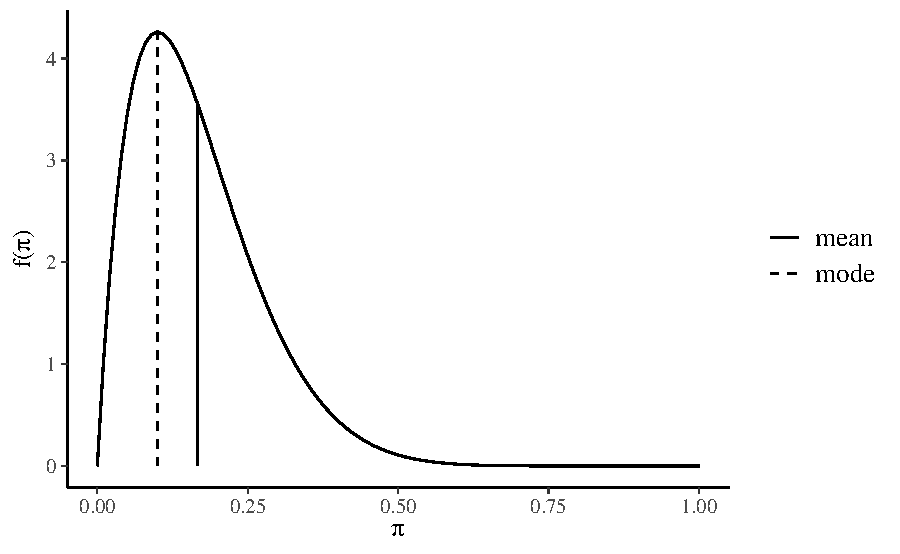
\includegraphics{ds4psy_files/figure-latex/unnamed-chunk-4-1} \end{center}

Tanto meglio la distribuzione \(q\) approssima la distribuzione target tanto più piccolo è il valore di divergenza KL.
\end{example}

\begin{example}
Sia \(p\) una distribuzione binomiale di parametri \(\theta = 0.2\) e \(n = 5\)

\begin{Shaded}
\begin{Highlighting}[]
\NormalTok{n }\OtherTok{\textless{}{-}} \DecValTok{4}
\NormalTok{p }\OtherTok{\textless{}{-}} \FloatTok{0.2}
\NormalTok{true\_py }\OtherTok{\textless{}{-}} \FunctionTok{dbinom}\NormalTok{(}\DecValTok{0}\SpecialCharTok{:}\NormalTok{n, n, }\FloatTok{0.2}\NormalTok{)}
\NormalTok{true\_py}
\CommentTok{\#\textgreater{} [1] 0.4096 0.4096 0.1536 0.0256 0.0016}
\end{Highlighting}
\end{Shaded}

\noindent Sia \(q_1\) una approssimazione a \(p\):

\begin{Shaded}
\begin{Highlighting}[]
\NormalTok{q1 }\OtherTok{\textless{}{-}} \FunctionTok{c}\NormalTok{(}\FloatTok{0.46}\NormalTok{, }\FloatTok{0.42}\NormalTok{, }\FloatTok{0.10}\NormalTok{, }\FloatTok{0.01}\NormalTok{, }\FloatTok{0.01}\NormalTok{)}
\NormalTok{q1}
\CommentTok{\#\textgreater{} [1] 0.46 0.42 0.10 0.01 0.01}
\end{Highlighting}
\end{Shaded}

Sia \(q_2\) una distribuzione uniforme:

\begin{Shaded}
\begin{Highlighting}[]
\NormalTok{q2 }\OtherTok{\textless{}{-}} \FunctionTok{rep}\NormalTok{(}\FloatTok{0.2}\NormalTok{, }\DecValTok{5}\NormalTok{)}
\NormalTok{q2}
\CommentTok{\#\textgreater{} [1] 0.2 0.2 0.2 0.2 0.2}
\end{Highlighting}
\end{Shaded}

La divergenza KL di \(q_1\) da \(p\) è

\begin{Shaded}
\begin{Highlighting}[]
\FunctionTok{sum}\NormalTok{(true\_py }\SpecialCharTok{*} \FunctionTok{log}\NormalTok{(true\_py }\SpecialCharTok{/}\NormalTok{ q1))}
\CommentTok{\#\textgreater{} [1] 0.02925}
\end{Highlighting}
\end{Shaded}

La divergenza KL di \(q_2\) da \(p\) è:

\begin{Shaded}
\begin{Highlighting}[]
\FunctionTok{sum}\NormalTok{(true\_py }\SpecialCharTok{*} \FunctionTok{log}\NormalTok{(true\_py }\SpecialCharTok{/}\NormalTok{ q2))}
\CommentTok{\#\textgreater{} [1] 0.4864}
\end{Highlighting}
\end{Shaded}

È chiaro che perdiamo una quantità maggiore di informazioni se, per descrivere la distribuzione binomiale \(p\), usiamo la distribuzione uniforme \(q_2\) anziché \(q_1\).
\end{example}

\hypertarget{la-divergenza-dipende-dalla-direzione}{%
\section{La divergenza dipende dalla direzione}\label{la-divergenza-dipende-dalla-direzione}}

La divergenza KL non è una vera e propria metrica: per esempio, non è simmetrica. In generale, \(\mathbb{KL}(p \mid\mid q) \neq \mathbb{KL}(q \mid\mid p)\), ovvero la \(\mathbb{KL}\) da \(p\) a \(q\) è diversa dalla \(\mathbb{KL}\) da \(q\) a \(p\).

\begin{example}

Usando le seguenti istruzioni \(\R\) otteniamo:

\begin{Shaded}
\begin{Highlighting}[]
\FunctionTok{tibble}\NormalTok{(}
  \AttributeTok{direction =} \FunctionTok{c}\NormalTok{(}\StringTok{"Da q a p"}\NormalTok{, }\StringTok{"Da p a q"}\NormalTok{),}
  \AttributeTok{p\_1 =} \FunctionTok{c}\NormalTok{(.}\DecValTok{01}\NormalTok{, .}\DecValTok{7}\NormalTok{),}
  \AttributeTok{q\_1 =} \FunctionTok{c}\NormalTok{(.}\DecValTok{7}\NormalTok{, .}\DecValTok{01}\NormalTok{)}
\NormalTok{) }\SpecialCharTok{\%\textgreater{}\%}
  \FunctionTok{mutate}\NormalTok{(}
    \AttributeTok{p\_2 =} \DecValTok{1} \SpecialCharTok{{-}}\NormalTok{ p\_1,}
    \AttributeTok{q\_2 =} \DecValTok{1} \SpecialCharTok{{-}}\NormalTok{ q\_1}
\NormalTok{  ) }\SpecialCharTok{\%\textgreater{}\%}
  \FunctionTok{mutate}\NormalTok{(}\AttributeTok{d\_kl =}\NormalTok{ (p\_1 }\SpecialCharTok{*} \FunctionTok{log}\NormalTok{(p\_1 }\SpecialCharTok{/}\NormalTok{ q\_1)) }\SpecialCharTok{+}\NormalTok{ (p\_2 }\SpecialCharTok{*} \FunctionTok{log}\NormalTok{(p\_2 }\SpecialCharTok{/}\NormalTok{ q\_2)))}
\CommentTok{\#\textgreater{} \# A tibble: 2 x 6}
\CommentTok{\#\textgreater{}   direction   p\_1   q\_1   p\_2   q\_2  d\_kl}
\CommentTok{\#\textgreater{}   \textless{}chr\textgreater{}     \textless{}dbl\textgreater{} \textless{}dbl\textgreater{} \textless{}dbl\textgreater{} \textless{}dbl\textgreater{} \textless{}dbl\textgreater{}}
\CommentTok{\#\textgreater{} 1 Da q a p   0.01  0.7   0.99  0.3   1.14}
\CommentTok{\#\textgreater{} 2 Da p a q   0.7   0.01  0.3   0.99  2.62}
\end{Highlighting}
\end{Shaded}

\end{example}

\hypertarget{confronto-tra-modelli}{%
\section{Confronto tra modelli}\label{confronto-tra-modelli}}

La divergenza KL viene utilizzata nel confronto tra modelli, ovvero ci consente di quantificare l'informazione che viene perduta quando utilizziamo la distribuzione di probabilità ipotizzata da un modello, chiamiamola \(p_{\mathcal{M}}\), per approssimare la distribuzione di probabilità del vero modello generatore dei dati, \(p_t\).

Nel Capitolo \ref{ch:intro-bayes-inference} abbiamo introdotto il concetto di distribuzione predittiva a posteriori:

\[
p(\tilde{y} \mid y) = \int_\Theta p(\tilde{y} \mid \theta) p(\theta \mid y) \,\operatorname {d}\!\theta .
\]

La distribuzione predittiva a posteriori descrive il tipo di dati che ci aspettiamo vengano prodotti dal modello generativo \(\mathcal{M}\), alla luce delle nostre credenze iniziali, \(p(\theta)\) e dei dati osservati \(y\). Quando valutiamo un modello ci chiediamo in che misura \(p_{\mathcal{M}}(\tilde{y} \mid y)\) approssimi \(p_t(\tilde{y})\). Cioè, ci chiediamo quanto siano simili i dati \(p_{\mathcal{M}}(\cdot)\) prodotti dal modello \(\mathcal{M}\) ai dati prodotti dal vero processo generatore dei dati \(p_t(\cdot)\).

Una misura della ``somiglianza'' tra la distribuzione \(q_{\mathcal{M}}\) ipotizzata dal modello \(\mathcal{M}\) e la distribuzione \(p_t\) del vero modello generatore dei dati è fornita dalla divergenza di Kullback-Leibler \(\mathbb{KL}(p_t \mid\mid q_{\mathcal{M}})\). Supponendo di avere \(k\) modelli della distribuzione a posteriori, \(\{q_{\mathcal{M}_1}, q_{\mathcal{M}_2}, \dots, q_{\mathcal{M}_k}\}\), e di conoscere il vero modello generatore dei dati, possiamo scrivere

\begin{align}
\mathbb{KL} (p_t \mid\mid q_{\mathcal{M}_1}) &= \E (\log p_{\mathcal{M}_0}) - \E (\log q_{\mathcal{M}_1})\notag\\
\mathbb{KL} (p_t \mid\mid q_{\mathcal{M}_2}) &= \E (\log p_t) - \E (\log q_{\mathcal{M}_2})\notag\\
&\cdots\notag\\
\mathbb{KL} (p_t \mid\mid q_{\mathcal{M}_k}) &= \E (\log p_{\mathcal{M}_0}) - \E (\log q_{\mathcal{M}_k}).
\label{eq:kl-mod-comp}
\end{align}

La \eqref{eq:kl-mod-comp} può sembrare un esercizio futile poiché nella vita reale non conosciamo il vero modello generatore dei dati. È però facile rendersi conto che, poiché \(p_t\) è la stessa per tutti i confronti, diventa possibile costruire un ordinamento dei modelli basato unicamente sul secondo termine della \eqref{eq:kl-mod-comp}, ovvero senza nessun riferimento al vero modello generatore dei dati. Per un generico modello \(\mathcal{M}\), il secondo termine della \eqref{eq:kl-mod-comp} può essere scritto come:

\begin{equation}
\E \log p_{\mathcal{M}}(y) = \int_{-\infty}^{+\infty}p_{t}(y)\log p_{\mathcal{M}}(y) \,\operatorname {d}\!y .
\label{eq:kl-div-cont-t2}
\end{equation}

\hypertarget{expected-log-predictive-density}{%
\section{Expected log predictive density}\label{expected-log-predictive-density}}

Le previsioni del modello \(\mathcal{M}\) sui nuovi dati futuri sono date dalla distribuzione predittiva a posteriori. Possiamo dunque riscrivere la \eqref{eq:kl-div-cont-t2} come

\begin{equation}
\elpd = \int_{\tilde{y}} p_{t}(\tilde{y}) \log p(\tilde{y} \mid y) \,\operatorname {d}\!\tilde{y}.
\label{eq:elpd}
\end{equation}

La \eqref{eq:elpd} è chiamata \emph{expected log predictive density} (\(\elpd\)) e fornisce la risposta al problema che ci eravamo posti: nel confronto tra modelli, come è possibile scegliere il modello più simile al vero meccanismo generatore dei dati? Possiamo pensare alla \eqref{eq:elpd} dicendo che descrive la distribuzione predittiva a posteriori del modello ponderando la verosimiglianza dei possibili (sconosciuti) dati futuri (\(\tilde{y}\)) con la vera distribuzione \(p_t\). Di conseguenza, valori \(\elpd\) più grandi identificano il modello che risulta più simile al vero meccanismo generatore dei dati.

Non dobbiamo preoccuparci di trovare una formulazione analitica della distribuzione predittiva a posteriori \(p(\tilde{y} \mid y)\) perché, come abbiamo visto nel Capitolo \ref{chapter-ppc}, è possibile approssimare tale distribuzione mediante simulazione. Notiamo però che la \eqref{eq:elpd} include un termine, \(p_t(\tilde{y})\), il quale descrive la distribuzione dei dati futuri \(\tilde{y}\) secondo il vero modello generatore dei dati. Il termine \(p_t\), ovviamente, è ignoto.\footnote{Se il modello sottostante i dati fosse noto non avremmo bisogno di cercare il modello migliore, perché \(p_t\) è il modello migliore.} Di conseguenza, la quantità \(\elpd\) non può mai essere calcolata in maniera esatta, ma può solo essere stimata. Il secondo problema di questo Capitolo è capire come la \eqref{eq:elpd} possa essere stimata utilizzando un campione di osservazioni.

\hypertarget{log-pointwise-predictive-density}{%
\subsection{Log pointwise predictive density}\label{log-pointwise-predictive-density}}

Ingenuamente, potremmo pensare di stimare la \eqref{eq:elpd} ipotizzando che la distribuzione del campione coincida con \(p_t\). Usare la distribuzione del campione come proxy del vero modello generatore dei dati (ovvero, ipotizzare che la distribuzione del campione rappresenti fedelmente \(p_t\)) comporta due conseguenze:

\begin{itemize}
\tightlist
\item
  non è necessario ponderare per \(p_t\), in quanto assumiamo che la distribuzione empirica del campione corrisponda a \(p_t\) (ciò significa assumere che i valori più comunemente osservati nel campione siano anche quelli più verosimili nella vera distribuzione \(p_t\));
\item
  dato che il campione è finito, anziché eseguire un'operazione di integrazione possiamo semplicemente sommare la densità predittiva a posteriori delle osservazioni.
\end{itemize}

Questo conduce alla seguente equazione:\footnote{In riferimento alla notazione, ricordiamo che \citet{gelman2014understanding} distinguono tra \(y^{rep}\) e \(\tilde{y}\). I valori \(y^{rep}\) corrispondono ad un'altra possibile realizzazione del medesimo modello statistico che ha prodotto \(y\) mediante determinati valori dei parametri \(\theta\) (repliche sotto lo stesso modello statistico). I valori \(\tilde{y}\) corrispondono invece ad un campione empirico di dati osservato in qualche futura occasione.}

\begin{equation}
\frac{1}{n} \sum_{i=1}^n \log p(y_i^{rep} \mid y).
\label{eq:1n-lppd}
\end{equation}

La quantità \eqref{eq:1n-lppd}, senza il passaggio finale della divisione per il numero di osservazioni, è chiamata \emph{log pointwise predictive density} (\(\lppd\))

\begin{equation}
\lppd = \sum_{i=1}^n \log p(y_i^{rep} \mid y)
\label{eq:lppd}
\end{equation}

e corrisponde alla somma delle densità predittive logaritmiche delle \(n\) osservazioni. Valori più grandi della \eqref{eq:lppd} sono da preferire perché indicano una maggiore accuratezza media. È anche comune vedere espressa la quantità precedente nei termini della \emph{devianza}, ovvero alla \(\lppd\) moltiplicata per -2. In questo secondo caso sono da preferire valori piccoli.

È importante notare che \(\lppd\) fornisce una \emph{sovrastima} della \eqref{eq:elpd}. Tale sovrastima è dovuta al fatto che, nel calcolo della \eqref{eq:lppd}, abbiamo usato \(p(y^{rep} \mid y)\) al posto di \(p(\tilde{y} \mid y)\): in altri termini, abbiamo considerato le osservazioni del campione come se fossero un nuovo campione di dati. In una serie di simulazioni, \citet{McElreath_rethinking} esamina il significato di questa sovrastima. Nelle simulazioni la devianza viene calcolata come funzione della complessità (ovvero, il numero di parametri) del modello. La simulazione mostra che \(\lppd\) aumenta al crescere del numero di parametri del modello. Ciò significa che \(\lppd\) mostra lo stesso limite del coefficiente di determinazione: aumenta all'aumentare della complessità del modello.

\begin{example}

Esaminiamo un esempio tratto da \href{https://vasishth.github.io/bayescogsci/book/expected-log-predictive-density-of-a-model.html}{Bayesian Data Analysis for Cognitive Science} nel quale la \(\elpd\) viene calcolata in forma esatta oppure mediante approssimazione. Supponiamo di disporre di un campione di \(n\) osservazioni. Supponiamo inoltre di conoscere il vero processo generativo dei dati (qualcosa che in pratica non è mai possibile), ovvero:

\[
p_t(y) = \Beta(1, 3).
\] I dati sono

\begin{Shaded}
\begin{Highlighting}[]
\FunctionTok{set.seed}\NormalTok{(}\DecValTok{75}\NormalTok{)}
\NormalTok{n }\OtherTok{\textless{}{-}} \DecValTok{10000}
\NormalTok{y\_data }\OtherTok{\textless{}{-}} \FunctionTok{rbeta}\NormalTok{(n, }\DecValTok{1}\NormalTok{, }\DecValTok{3}\NormalTok{)}
\FunctionTok{head}\NormalTok{(y\_data)}
\CommentTok{\#\textgreater{} [1] 0.55062 0.13346 0.80251 0.21431 0.01913 0.08677}
\end{Highlighting}
\end{Shaded}

Supponiamo inoltre di avere adattato ai dati un modello bayesiano \(\mathcal{M}\) e di avere ottenuto la distribuzione a posteriori per i parametri del modello. Inoltre, supponiamo di avere derivato la forma analitica della distribuzione predittiva a posteriori per il modello:

\[
p(y^{rep} \mid y) \sim \Beta(2, 2).
\]

Questa distribuzione ci dice quanto sono credibili i possibili dati futuri.

Conoscendo la vera distribuzione dei dati \(p_t(y)\) possiamo calcolare in forma esatta la quantità \(\elpd\), ovvero

\[
\elpd = \int_{y^{rep}}p_{t}(y^{rep})\log p(y^{rep} \mid y) \,\operatorname {d}\!y^{rep}.
\]

Svolgiamo i calcoli in \(\R\) otteniamo:

\begin{Shaded}
\begin{Highlighting}[]
\CommentTok{\# True distribution}
\NormalTok{p\_t }\OtherTok{\textless{}{-}} \ControlFlowTok{function}\NormalTok{(y) }\FunctionTok{dbeta}\NormalTok{(y, }\DecValTok{1}\NormalTok{, }\DecValTok{3}\NormalTok{)}
\CommentTok{\# Predictive distribution}
\NormalTok{p }\OtherTok{\textless{}{-}} \ControlFlowTok{function}\NormalTok{(y) }\FunctionTok{dbeta}\NormalTok{(y, }\DecValTok{2}\NormalTok{, }\DecValTok{2}\NormalTok{)}
\CommentTok{\# Integration}
\NormalTok{integrand }\OtherTok{\textless{}{-}} \ControlFlowTok{function}\NormalTok{(y) }\FunctionTok{p\_t}\NormalTok{(y) }\SpecialCharTok{*} \FunctionTok{log}\NormalTok{(}\FunctionTok{p}\NormalTok{(y))}
\FunctionTok{integrate}\NormalTok{(}\AttributeTok{f =}\NormalTok{ integrand, }\AttributeTok{lower =} \DecValTok{0}\NormalTok{, }\AttributeTok{upper =} \DecValTok{1}\NormalTok{)}
\CommentTok{\#\textgreater{} {-}0.3749 with absolute error \textless{} 6.8e{-}07}
\end{Highlighting}
\end{Shaded}

Tuttavia, in pratica non conosciamo mai \(p_t(y)\). Quindi approssimiamo \(\elpd\) usando la \eqref{eq:elpd}:

\[
\frac{1}{n} \sum_{i=1}^n \log p(y_i \mid y).
\]

Così facendo, e svolgendo i calcoli in \(\R\), otteniamo un valore diverso da quello trovato in precedenza:

\begin{Shaded}
\begin{Highlighting}[]
\DecValTok{1} \SpecialCharTok{/}\NormalTok{ n }\SpecialCharTok{*} \FunctionTok{sum}\NormalTok{(}\FunctionTok{log}\NormalTok{(}\FunctionTok{p}\NormalTok{(y\_data)))}
\CommentTok{\#\textgreater{} [1] {-}0.3639}
\end{Highlighting}
\end{Shaded}

\end{example}

\hypertarget{commenti-e-considerazioni-finali}{%
\section*{Commenti e considerazioni finali}\label{commenti-e-considerazioni-finali}}


Dato che non conosciamo il vero meccanismo generatore dei dati \(p\), possiamo usare la distribuzione dei dati osservata come proxy per la vera distribuzione \(p\). Quindi, invece di ponderare la distribuzione predittiva in base alla densità reale di tutti i possibili dati futuri, utilizziamo semplicemente le \(n\) osservazioni che abbiamo. Possiamo farlo perché assumiamo che le nostre osservazioni costituiscano un campione dalla vera distribuzione dei dati: in base a questa ipotesi, nel campione ci aspettiamo di osservare più frequentemente quelle osservazioni che hanno una maggiore verosimiglianza nella vera distribuzione \(p\). È così possibile giungere ad una stima numerica della \(\elpd\) chiamata \emph{log pointwise predictive density} (\(\lppd\)).

  \bibliography{refs.bib,book.bib,packages.bib}

\printindex

\end{document}
